\begin{figure}[htbp]
\centering
\resizebox{\textwidth}{!}{%
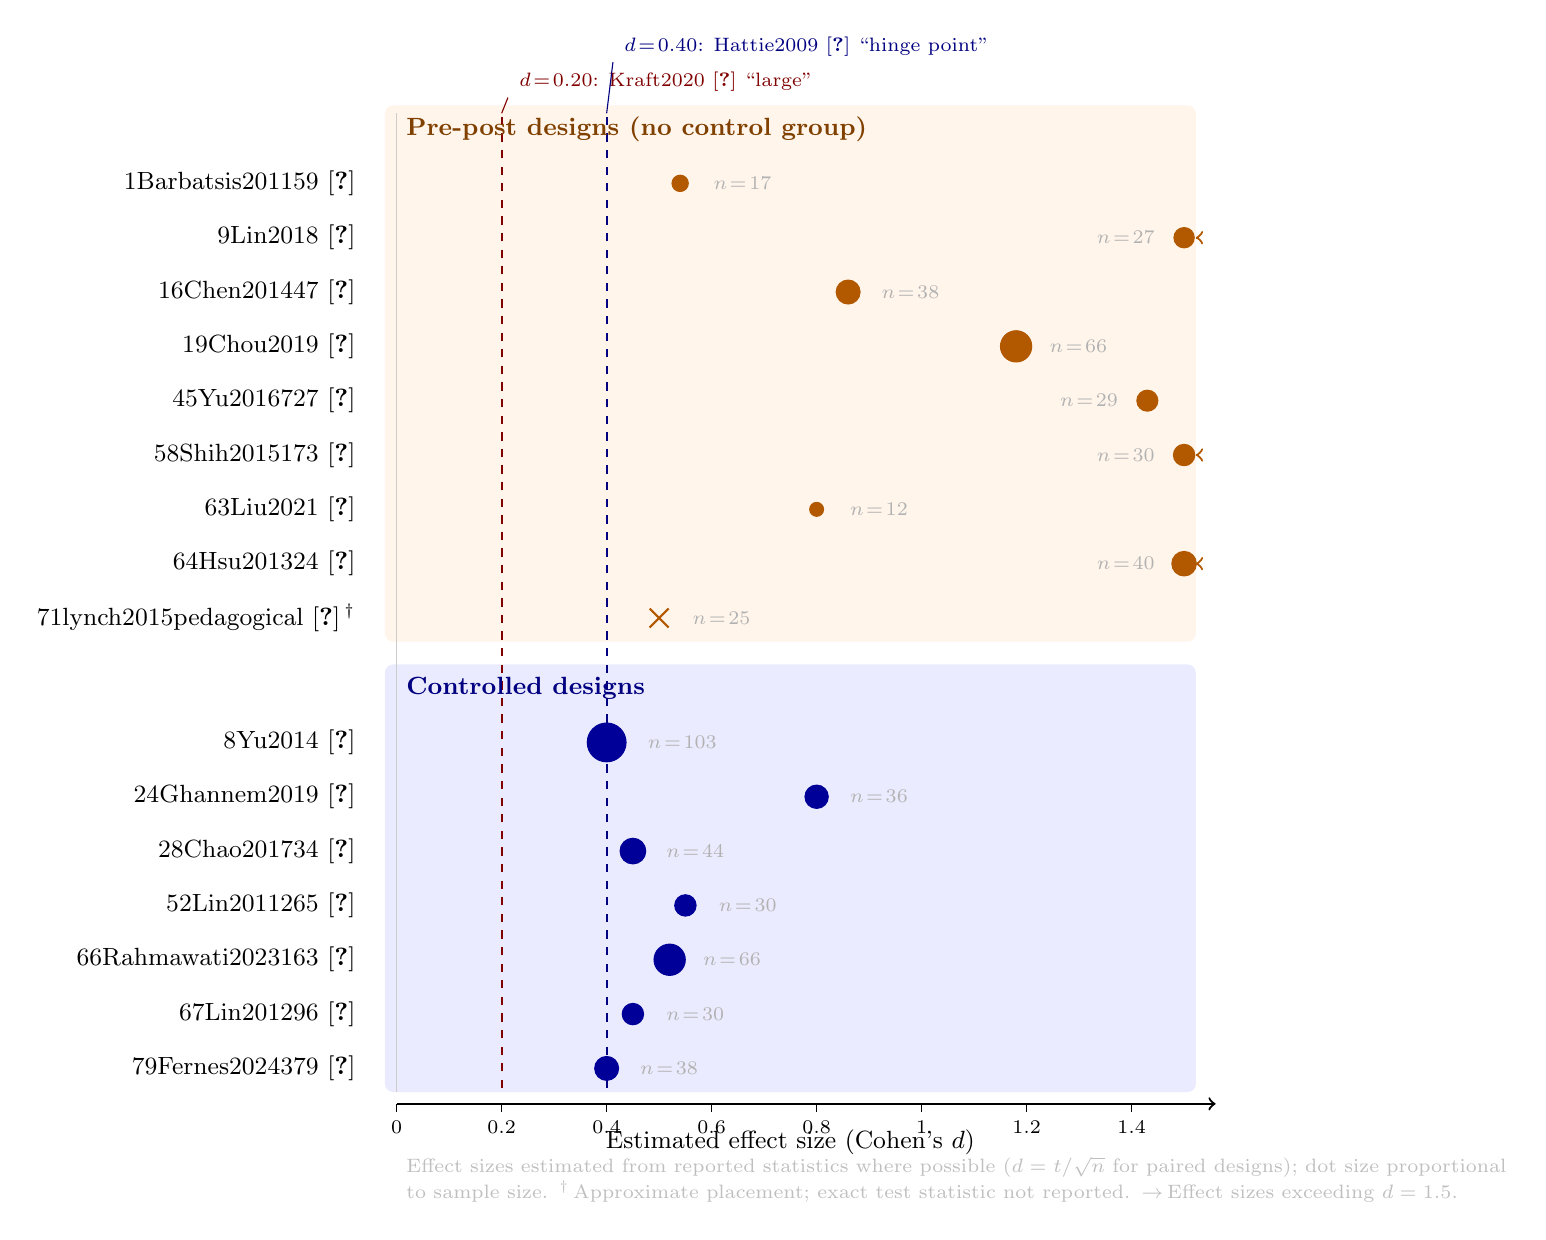
\begin{tikzpicture}[
    every node/.style={font=\small},
    prepost/.style={fill=orange!70!black, draw=orange!70!black},
    controlled/.style={fill=blue!60!black, draw=blue!60!black},
]

% --- Layout parameters ---
\def\plotleft{0}
\def\plotright{10.0}      % x-axis length in cm for d range [0, 1.5]
\def\labelright{-0.4}     % right edge of study labels
\def\rowsep{0.69}         % vertical spacing between rows

% Scaling: d value -> x position in cm
\pgfmathsetmacro{\xscale}{\plotright/1.5}

% --- Y positions (top to bottom) ---
% Group header: Pre-post
\def\headerPrePost{12.58}
% Pre-post studies (9 rows)
\def\yA{11.89}  % Barbatsis et al. 2011
\def\yB{11.20}  % Lin et al. 2018
\def\yC{10.51}  % Chen et al. 2014
\def\yD{9.82}   % Chou et al. 2019
\def\yE{9.13}   % Yu et al. 2016
\def\yF{8.44}   % Shih et al. 2015
\def\yG{7.75}   % Liu et al. 2021
\def\yH{7.06}   % Hsu et al. 2013
\def\yI{6.37}   % Lynch et al. 2015

% Group header: Controlled
\def\headerControlled{5.48}
% Controlled studies (7 rows)
\def\yJ{4.79}   % Yu et al. 2014
\def\yK{4.10}   % Ghannem et al. 2019
\def\yL{3.41}   % Chao et al. 2017
\def\yM{2.72}   % Lin \& Wei 2011
\def\yN{2.03}   % Rahmawati et al. 2023
\def\yO{1.34}   % Lin et al. 2012
\def\yP{0.65}   % Fernes et al. 2024

% --- Background shading for groups ---
\fill[orange!8, rounded corners=3pt]
    (\plotleft-0.15, \yI-0.30) rectangle (\plotright+0.15, \headerPrePost+0.30);
\fill[blue!8, rounded corners=3pt]
    (\plotleft-0.15, \yP-0.30) rectangle (\plotright+0.15, \headerControlled+0.30);

% --- Vertical benchmark lines ---
% d = 0.20 (Kraft threshold)
\pgfmathsetmacro{\xKraft}{0.20*\xscale}
\draw[red!50!black, dashed, thick]
    (\xKraft, \yP-0.25) -- (\xKraft, \headerPrePost+0.20);

% d = 0.40 (Hattie hinge point)
\pgfmathsetmacro{\xHattie}{0.40*\xscale}
\draw[blue!50!black, dashed, thick]
    (\xHattie, \yP-0.25) -- (\xHattie, \headerPrePost+0.20);

% --- Benchmark labels at top (horizontal, no overlap) ---
\node[font=\scriptsize, text=red!50!black, anchor=south west]
    at (\xKraft+0.1, \headerPrePost+0.35)
    {$d\!=\!0.20$: \citeauthor{Kraft2020}~\cite{Kraft2020} ``large''};
\node[font=\scriptsize, text=blue!50!black, anchor=south west]
    at (\xHattie+0.1, \headerPrePost+0.80)
    {$d\!=\!0.40$: \citeauthor{Hattie2009}~\cite{Hattie2009} ``hinge point''};
% Small connector lines from labels to dashed lines
\draw[red!50!black, thin] (\xKraft, \headerPrePost+0.20) -- (\xKraft+0.08, \headerPrePost+0.40);
\draw[blue!50!black, thin] (\xHattie, \headerPrePost+0.20) -- (\xHattie+0.08, \headerPrePost+0.85);

% --- X-axis ---
\draw[thick, ->] (\plotleft, \yP-0.45) -- (\plotright+0.4, \yP-0.45);
\node[font=\small, anchor=north] at (\plotright/2, \yP-0.65) {Estimated effect size (Cohen's $d$)};
% Tick marks
\foreach \d in {0, 0.2, 0.4, 0.6, 0.8, 1.0, 1.2, 1.4} {
    \pgfmathsetmacro{\xt}{\d*\xscale}
    \draw (\xt, \yP-0.45) -- (\xt, \yP-0.55);
    \node[font=\scriptsize, anchor=north] at (\xt, \yP-0.55) {\pgfmathprintnumber[fixed, precision=1]{\d}};
}

% --- Zero line ---
\draw[gray!40, thin] (\plotleft, \yP-0.30) -- (\plotleft, \headerPrePost+0.20);

% --- Group headers ---
\node[font=\small\bfseries, anchor=west, text=orange!50!black]
    at (\plotleft, \headerPrePost) {Pre-post designs (no control group)};
\node[font=\small\bfseries, anchor=west, text=blue!50!black]
    at (\plotleft, \headerControlled) {Controlled designs};

% =====================================================================
% PRE-POST STUDIES
% =====================================================================

% 1. Barbatsis et al. 2011, n=17, d=0.54
\node[font=\small, anchor=east] at (\labelright, \yA) {\citeauthor{1Barbatsis201159}~\cite{1Barbatsis201159}};
\pgfmathsetmacro{\xdot}{0.54*\xscale}
\pgfmathsetmacro{\rdot}{2.5 + 4.5*(sqrt(17)-sqrt(12))/(sqrt(103)-sqrt(12))}
\fill[prepost] (\xdot, \yA) circle (\rdot pt);
\node[font=\scriptsize, anchor=west, text=gray!60] at (\xdot+0.3, \yA) {$n\!=\!17$};

% 2. Lin et al. 2018, n=27, d>1.5 (capped)
\node[font=\small, anchor=east] at (\labelright, \yB) {\citeauthor{9Lin2018}~\cite{9Lin2018}};
\pgfmathsetmacro{\xdot}{1.50*\xscale}
\pgfmathsetmacro{\rdot}{2.5 + 4.5*(sqrt(27)-sqrt(12))/(sqrt(103)-sqrt(12))}
\fill[prepost] (\xdot, \yB) circle (\rdot pt);
\draw[orange!70!black, thick, ->] (\xdot+0.15, \yB) -- (\plotright+0.15, \yB);
\node[font=\scriptsize, anchor=east, text=gray!60] at (\xdot-0.25, \yB) {$n\!=\!27$};

% 3. Chen et al. 2014, n=38, d=0.86
\node[font=\small, anchor=east] at (\labelright, \yC) {\citeauthor{16Chen201447}~\cite{16Chen201447}};
\pgfmathsetmacro{\xdot}{0.86*\xscale}
\pgfmathsetmacro{\rdot}{2.5 + 4.5*(sqrt(38)-sqrt(12))/(sqrt(103)-sqrt(12))}
\fill[prepost] (\xdot, \yC) circle (\rdot pt);
\node[font=\scriptsize, anchor=west, text=gray!60] at (\xdot+0.3, \yC) {$n\!=\!38$};

% 4. Chou et al. 2019, n=66, d=1.18
\node[font=\small, anchor=east] at (\labelright, \yD) {\citeauthor{19Chou2019}~\cite{19Chou2019}};
\pgfmathsetmacro{\xdot}{1.18*\xscale}
\pgfmathsetmacro{\rdot}{2.5 + 4.5*(sqrt(66)-sqrt(12))/(sqrt(103)-sqrt(12))}
\fill[prepost] (\xdot, \yD) circle (\rdot pt);
\node[font=\scriptsize, anchor=west, text=gray!60] at (\xdot+0.3, \yD) {$n\!=\!66$};

% 5. Yu et al. 2016, n=29, d=1.43
\node[font=\small, anchor=east] at (\labelright, \yE) {\citeauthor{45Yu2016727}~\cite{45Yu2016727}};
\pgfmathsetmacro{\xdot}{1.43*\xscale}
\pgfmathsetmacro{\rdot}{2.5 + 4.5*(sqrt(29)-sqrt(12))/(sqrt(103)-sqrt(12))}
\fill[prepost] (\xdot, \yE) circle (\rdot pt);
\node[font=\scriptsize, anchor=east, text=gray!60] at (\xdot-0.25, \yE) {$n\!=\!29$};

% 6. Shih et al. 2015, n=30, d>1.5 (capped)
\node[font=\small, anchor=east] at (\labelright, \yF) {\citeauthor{58Shih2015173}~\cite{58Shih2015173}};
\pgfmathsetmacro{\xdot}{1.50*\xscale}
\pgfmathsetmacro{\rdot}{2.5 + 4.5*(sqrt(30)-sqrt(12))/(sqrt(103)-sqrt(12))}
\fill[prepost] (\xdot, \yF) circle (\rdot pt);
\draw[orange!70!black, thick, ->] (\xdot+0.15, \yF) -- (\plotright+0.15, \yF);
\node[font=\scriptsize, anchor=east, text=gray!60] at (\xdot-0.25, \yF) {$n\!=\!30$};

% 7. Liu et al. 2021, n=12, d=0.80
\node[font=\small, anchor=east] at (\labelright, \yG) {\citeauthor{63Liu2021}~\cite{63Liu2021}};
\pgfmathsetmacro{\xdot}{0.80*\xscale}
\fill[prepost] (\xdot, \yG) circle (2.5pt);
\node[font=\scriptsize, anchor=west, text=gray!60] at (\xdot+0.3, \yG) {$n\!=\!12$};

% 8. Hsu et al. 2013, n=40, d>1.5 (capped)
\node[font=\small, anchor=east] at (\labelright, \yH) {\citeauthor{64Hsu201324}~\cite{64Hsu201324}};
\pgfmathsetmacro{\xdot}{1.50*\xscale}
\pgfmathsetmacro{\rdot}{2.5 + 4.5*(sqrt(40)-sqrt(12))/(sqrt(103)-sqrt(12))}
\fill[prepost] (\xdot, \yH) circle (\rdot pt);
\draw[orange!70!black, thick, ->] (\xdot+0.15, \yH) -- (\plotright+0.15, \yH);
\node[font=\scriptsize, anchor=east, text=gray!60] at (\xdot-0.25, \yH) {$n\!=\!40$};

% 9. Lynch et al. 2015, n=25, d~0.50 (approximate)
\node[font=\small, anchor=east] at (\labelright, \yI) {\citeauthor{71lynch2015pedagogical}~\cite{71lynch2015pedagogical}\,\textsuperscript{$\dagger$}};
\pgfmathsetmacro{\xdot}{0.50*\xscale}
\draw[prepost, thick] (\xdot-0.12, \yI-0.12) -- (\xdot+0.12, \yI+0.12);
\draw[prepost, thick] (\xdot-0.12, \yI+0.12) -- (\xdot+0.12, \yI-0.12);
\node[font=\scriptsize, anchor=west, text=gray!60] at (\xdot+0.3, \yI) {$n\!=\!25$};

% =====================================================================
% CONTROLLED STUDIES
% =====================================================================

% 10. Yu et al. 2014, n=103, d=0.40
\node[font=\small, anchor=east] at (\labelright, \yJ) {\citeauthor{8Yu2014}~\cite{8Yu2014}};
\pgfmathsetmacro{\xdot}{0.40*\xscale}
\fill[controlled] (\xdot, \yJ) circle (7pt);
\node[font=\scriptsize, anchor=west, text=gray!60] at (\xdot+0.4, \yJ) {$n\!=\!103$};

% 11. Ghannem et al. 2019, n=36, d=0.80
\node[font=\small, anchor=east] at (\labelright, \yK) {\citeauthor{24Ghannem2019}~\cite{24Ghannem2019}};
\pgfmathsetmacro{\xdot}{0.80*\xscale}
\pgfmathsetmacro{\rdot}{2.5 + 4.5*(sqrt(36)-sqrt(12))/(sqrt(103)-sqrt(12))}
\fill[controlled] (\xdot, \yK) circle (\rdot pt);
\node[font=\scriptsize, anchor=west, text=gray!60] at (\xdot+0.3, \yK) {$n\!=\!36$};

% 12. Chao et al. 2017, n=44, d=0.45
\node[font=\small, anchor=east] at (\labelright, \yL) {\citeauthor{28Chao201734}~\cite{28Chao201734}};
\pgfmathsetmacro{\xdot}{0.45*\xscale}
\pgfmathsetmacro{\rdot}{2.5 + 4.5*(sqrt(44)-sqrt(12))/(sqrt(103)-sqrt(12))}
\fill[controlled] (\xdot, \yL) circle (\rdot pt);
\node[font=\scriptsize, anchor=west, text=gray!60] at (\xdot+0.3, \yL) {$n\!=\!44$};

% 13. Lin \& Wei 2011, n=30, d=0.55
\node[font=\small, anchor=east] at (\labelright, \yM) {\citeauthor{52Lin2011265}~\cite{52Lin2011265}};
\pgfmathsetmacro{\xdot}{0.55*\xscale}
\pgfmathsetmacro{\rdot}{2.5 + 4.5*(sqrt(30)-sqrt(12))/(sqrt(103)-sqrt(12))}
\fill[controlled] (\xdot, \yM) circle (\rdot pt);
\node[font=\scriptsize, anchor=west, text=gray!60] at (\xdot+0.3, \yM) {$n\!=\!30$};

% 14. Rahmawati et al. 2023, n=66, d=0.52
\node[font=\small, anchor=east] at (\labelright, \yN) {\citeauthor{66Rahmawati2023163}~\cite{66Rahmawati2023163}};
\pgfmathsetmacro{\xdot}{0.52*\xscale}
\pgfmathsetmacro{\rdot}{2.5 + 4.5*(sqrt(66)-sqrt(12))/(sqrt(103)-sqrt(12))}
\fill[controlled] (\xdot, \yN) circle (\rdot pt);
\node[font=\scriptsize, anchor=west, text=gray!60] at (\xdot+0.3, \yN) {$n\!=\!66$};

% 15. Lin et al. 2012, n=30, d=0.45
\node[font=\small, anchor=east] at (\labelright, \yO) {\citeauthor{67Lin201296}~\cite{67Lin201296}};
\pgfmathsetmacro{\xdot}{0.45*\xscale}
\pgfmathsetmacro{\rdot}{2.5 + 4.5*(sqrt(30)-sqrt(12))/(sqrt(103)-sqrt(12))}
\fill[controlled] (\xdot, \yO) circle (\rdot pt);
\node[font=\scriptsize, anchor=west, text=gray!60] at (\xdot+0.3, \yO) {$n\!=\!30$};

% 16. Fernes et al. 2024, n=38, d=0.40
\node[font=\small, anchor=east] at (\labelright, \yP) {\citeauthor{79Fernes2024379}~\cite{79Fernes2024379}};
\pgfmathsetmacro{\xdot}{0.40*\xscale}
\pgfmathsetmacro{\rdot}{2.5 + 4.5*(sqrt(38)-sqrt(12))/(sqrt(103)-sqrt(12))}
\fill[controlled] (\xdot, \yP) circle (\rdot pt);
\node[font=\scriptsize, anchor=west, text=gray!60] at (\xdot+0.3, \yP) {$n\!=\!38$};

% --- Footnote ---
\node[font=\scriptsize, text=gray!50, anchor=north west, text width=14cm]
    at (\plotleft, \yP-1.0) {%
    Effect sizes estimated from reported statistics where possible ($d = t/\sqrt{n}$ for paired designs); dot size proportional to sample size.
    \textsuperscript{$\dagger$}\,Approximate placement; exact test statistic not reported.
    $\rightarrow$\,Effect sizes exceeding $d = 1.5$.};

\end{tikzpicture}%
}% end resizebox
\caption{Forest-plot summary of 16 studies reporting statistically significant learning outcomes, grouped by study design. Vertical benchmark lines indicate the threshold for ``large'' effects in scalable educational interventions ($d = 0.20$) proposed by \citeauthor{Kraft2020}~\cite{Kraft2020} and the ``hinge point'' ($d = 0.40$) identified by \citeauthor{Hattie2009}~\cite{Hattie2009}.}
\label{fig:effect-size-forest}
\end{figure}
